
%% bare_conf_compsoc.tex
%% V1.4b
%% 2015/08/26
%% by Michael Shell
%% See:
%% http://www.michaelshell.org/
%% for current contact information.
%%
%% This is a skeleton file demonstrating the use of IEEEtran.cls
%% (requires IEEEtran.cls version 1.8b or later) with an IEEE Computer
%% Society conference paper.
%%
%% Support sites:
%% http://www.michaelshell.org/tex/ieeetran/
%% http://www.ctan.org/pkg/ieeetran
%% and
%% http://www.ieee.org/

%%*************************************************************************
%% Legal Notice:
%% This code is offered as-is without any warranty either expressed or
%% implied; without even the implied warranty of MERCHANTABILITY or
%% FITNESS FOR A PARTICULAR PURPOSE! 
%% User assumes all risk.
%% In no event shall the IEEE or any contributor to this code be liable for
%% any damages or losses, including, but not limited to, incidental,
%% consequential, or any other damages, resulting from the use or misuse
%% of any information contained here.
%%
%% All comments are the opinions of their respective authors and are not
%% necessarily endorsed by the IEEE.
%%
%% This work is distributed under the LaTeX Project Public License (LPPL)
%% ( http://www.latex-project.org/ ) version 1.3, and may be freely used,
%% distributed and modified. A copy of the LPPL, version 1.3, is included
%% in the base LaTeX documentation of all distributions of LaTeX released
%% 2003/12/01 or later.
%% Retain all contribution notices and credits.
%% ** Modified files should be clearly indicated as such, including  **
%% ** renaming them and changing author support contact information. **
%%*************************************************************************


% *** Authors should verify (and, if needed, correct) their LaTeX system  ***
% *** with the testflow diagnostic prior to trusting their LaTeX platform ***
% *** with production work. The IEEE's font choices and paper sizes can   ***
% *** trigger bugs that do not appear when using other class files.       ***                          ***
% The testflow support page is at:
% http://www.michaelshell.org/tex/testflow/



\documentclass[conference,compsoc]{IEEEtran}
% Some/most Computer Society conferences require the compsoc mode option,
% but others may want the standard conference format.
%
% If IEEEtran.cls has not been installed into the LaTeX system files,
% manually specify the path to it like:
% \documentclass[conference,compsoc]{../sty/IEEEtran}





% Some very useful LaTeX packages include:
% (uncomment the ones you want to load)


% *** MISC UTILITY PACKAGES ***
%
%\usepackage{ifpdf}
% Heiko Oberdiek's ifpdf.sty is very useful if you need conditional
% compilation based on whether the output is pdf or dvi.
% usage:
% \ifpdf
%   % pdf code
% \else
%   % dvi code
% \fi
% The latest version of ifpdf.sty can be obtained from:
% http://www.ctan.org/pkg/ifpdf
% Also, note that IEEEtran.cls V1.7 and later provides a builtin
% \ifCLASSINFOpdf conditional that works the same way.
% When switching from latex to pdflatex and vice-versa, the compiler may
% have to be run twice to clear warning/error messages.






% *** CITATION PACKAGES ***
%
\usepackage{graphicx}
\ifCLASSOPTIONcompsoc
  % IEEE Computer Society needs nocompress option
  % requires cite.sty v4.0 or later (November 2003)
  \usepackage[nocompress]{cite}
\else
  % normal IEEE
  \usepackage{cite}
\fi
% cite.sty was written by Donald Arseneau
% V1.6 and later of IEEEtran pre-defines the format of the cite.sty package
% \cite{} output to follow that of the IEEE. Loading the cite package will
% result in citation numbers being automatically sorted and properly
% "compressed/ranged". e.g., [1], [9], [2], [7], [5], [6] without using
% cite.sty will become [1], [2], [5]--[7], [9] using cite.sty. cite.sty's
% \cite will automatically add leading space, if needed. Use cite.sty's
% noadjust option (cite.sty V3.8 and later) if you want to turn this off
% such as if a citation ever needs to be enclosed in parenthesis.
% cite.sty is already installed on most LaTeX systems. Be sure and use
% version 5.0 (2009-03-20) and later if using hyperref.sty.
% The latest version can be obtained at:
% http://www.ctan.org/pkg/cite
% The documentation is contained in the cite.sty file itself.
%
% Note that some packages require special options to format as the Computer
% Society requires. In particular, Computer Society  papers do not use
% compressed citation ranges as is done in typical IEEE papers
% (e.g., [1]-[4]). Instead, they list every citation separately in order
% (e.g., [1], [2], [3], [4]). To get the latter we need to load the cite
% package with the nocompress option which is supported by cite.sty v4.0
% and later.





% *** GRAPHICS RELATED PACKAGES ***
%
\ifCLASSINFOpdf
  % \usepackage[pdftex]{graphicx}
  % declare the path(s) where your graphic files are
  % \graphicspath{{../pdf/}{../jpeg/}}
  % and their extensions so you won't have to specify these with
  % every instance of \includegraphics
  % \DeclareGraphicsExtensions{.pdf,.jpeg,.png}
\else
  % or other class option (dvipsone, dvipdf, if not using dvips). graphicx
  % will default to the driver specified in the system graphics.cfg if no
  % driver is specified.
  % \usepackage[dvips]{graphicx}
  % declare the path(s) where your graphic files are
  % \graphicspath{{../eps/}}
  % and their extensions so you won't have to specify these with
  % every instance of \includegraphics
  % \DeclareGraphicsExtensions{.eps}
\fi
% graphicx was written by David Carlisle and Sebastian Rahtz. It is
% required if you want graphics, photos, etc. graphicx.sty is already
% installed on most LaTeX systems. The latest version and documentation
% can be obtained at: 
% http://www.ctan.org/pkg/graphicx
% Another good source of documentation is "Using Imported Graphics in
% LaTeX2e" by Keith Reckdahl which can be found at:
% http://www.ctan.org/pkg/epslatex
%
% latex, and pdflatex in dvi mode, support graphics in encapsulated
% postscript (.eps) format. pdflatex in pdf mode supports graphics
% in .pdf, .jpeg, .png and .mps (metapost) formats. Users should ensure
% that all non-photo figures use a vector format (.eps, .pdf, .mps) and
% not a bitmapped formats (.jpeg, .png). The IEEE frowns on bitmapped formats
% which can result in "jaggedy"/blurry rendering of lines and letters as
% well as large increases in file sizes.
%
% You can find documentation about the pdfTeX application at:
% http://www.tug.org/applications/pdftex





% *** MATH PACKAGES ***
%
%\usepackage{amsmath}
% A popular package from the American Mathematical Society that provides
% many useful and powerful commands for dealing with mathematics.
%
% Note that the amsmath package sets \interdisplaylinepenalty to 10000
% thus preventing page breaks from occurring within multiline equations. Use:
%\interdisplaylinepenalty=2500
% after loading amsmath to restore such page breaks as IEEEtran.cls normally
% does. amsmath.sty is already installed on most LaTeX systems. The latest
% version and documentation can be obtained at:
% http://www.ctan.org/pkg/amsmath





% *** SPECIALIZED LIST PACKAGES ***
%
%\usepackage{algorithmic}
% algorithmic.sty was written by Peter Williams and Rogerio Brito.
% This package provides an algorithmic environment fo describing algorithms.
% You can use the algorithmic environment in-text or within a figure
% environment to provide for a floating algorithm. Do NOT use the algorithm
% floating environment provided by algorithm.sty (by the same authors) or
% algorithm2e.sty (by Christophe Fiorio) as the IEEE does not use dedicated
% algorithm float types and packages that provide these will not provide
% correct IEEE style captions. The latest version and documentation of
% algorithmic.sty can be obtained at:
% http://www.ctan.org/pkg/algorithms
% Also of interest may be the (relatively newer and more customizable)
% algorithmicx.sty package by Szasz Janos:
% http://www.ctan.org/pkg/algorithmicx




% *** ALIGNMENT PACKAGES ***
%
%\usepackage{array}
% Frank Mittelbach's and David Carlisle's array.sty patches and improves
% the standard LaTeX2e array and tabular environments to provide better
% appearance and additional user controls. As the default LaTeX2e table
% generation code is lacking to the point of almost being broken with
% respect to the quality of the end results, all users are strongly
% advised to use an enhanced (at the very least that provided by array.sty)
% set of table tools. array.sty is already installed on most systems. The
% latest version and documentation can be obtained at:
% http://www.ctan.org/pkg/array


% IEEEtran contains the IEEEeqnarray family of commands that can be used to
% generate multiline equations as well as matrices, tables, etc., of high
% quality.




% *** SUBFIGURE PACKAGES ***
%\ifCLASSOPTIONcompsoc
%  \usepackage[caption=false,font=footnotesize,labelfont=sf,textfont=sf]{subfig}
%\else
%  \usepackage[caption=false,font=footnotesize]{subfig}
%\fi
% subfig.sty, written by Steven Douglas Cochran, is the modern replacement
% for subfigure.sty, the latter of which is no longer maintained and is
% incompatible with some LaTeX packages including fixltx2e. However,
% subfig.sty requires and automatically loads Axel Sommerfeldt's caption.sty
% which will override IEEEtran.cls' handling of captions and this will result
% in non-IEEE style figure/table captions. To prevent this problem, be sure
% and invoke subfig.sty's "caption=false" package option (available since
% subfig.sty version 1.3, 2005/06/28) as this is will preserve IEEEtran.cls
% handling of captions.
% Note that the Computer Society format requires a sans serif font rather
% than the serif font used in traditional IEEE formatting and thus the need
% to invoke different subfig.sty package options depending on whether
% compsoc mode has been enabled.
%
% The latest version and documentation of subfig.sty can be obtained at:
% http://www.ctan.org/pkg/subfig




% *** FLOAT PACKAGES ***
%
%\usepackage{fixltx2e}
% fixltx2e, the successor to the earlier fix2col.sty, was written by
% Frank Mittelbach and David Carlisle. This package corrects a few problems
% in the LaTeX2e kernel, the most notable of which is that in current
% LaTeX2e releases, the ordering of single and double column floats is not
% guaranteed to be preserved. Thus, an unpatched LaTeX2e can allow a
% single column figure to be placed prior to an earlier double column
% figure.
% Be aware that LaTeX2e kernels dated 2015 and later have fixltx2e.sty's
% corrections already built into the system in which case a warning will
% be issued if an attempt is made to load fixltx2e.sty as it is no longer
% needed.
% The latest version and documentation can be found at:
% http://www.ctan.org/pkg/fixltx2e


%\usepackage{stfloats}
% stfloats.sty was written by Sigitas Tolusis. This package gives LaTeX2e
% the ability to do double column floats at the bottom of the page as well
% as the top. (e.g., "\begin{figure*}[!b]" is not normally possible in
% LaTeX2e). It also provides a command:
%\fnbelowfloat
% to enable the placement of footnotes below bottom floats (the standard
% LaTeX2e kernel puts them above bottom floats). This is an invasive package
% which rewrites many portions of the LaTeX2e float routines. It may not work
% with other packages that modify the LaTeX2e float routines. The latest
% version and documentation can be obtained at:
% http://www.ctan.org/pkg/stfloats
% Do not use the stfloats baselinefloat ability as the IEEE does not allow
% \baselineskip to stretch. Authors submitting work to the IEEE should note
% that the IEEE rarely uses double column equations and that authors should try
% to avoid such use. Do not be tempted to use the cuted.sty or midfloat.sty
% packages (also by Sigitas Tolusis) as the IEEE does not format its papers in
% such ways.
% Do not attempt to use stfloats with fixltx2e as they are incompatible.
% Instead, use Morten Hogholm'a dblfloatfix which combines the features
% of both fixltx2e and stfloats:
%
% \usepackage{dblfloatfix}
% The latest version can be found at:
% http://www.ctan.org/pkg/dblfloatfix




% *** PDF, URL AND HYPERLINK PACKAGES ***
%
%\usepackage{url}
% url.sty was written by Donald Arseneau. It provides better support for
% handling and breaking URLs. url.sty is already installed on most LaTeX
% systems. The latest version and documentation can be obtained at:
% http://www.ctan.org/pkg/url
% Basically, \url{my_url_here}.




% *** Do not adjust lengths that control margins, column widths, etc. ***
% *** Do not use packages that alter fonts (such as pslatex).         ***
% There should be no need to do such things with IEEEtran.cls V1.6 and later.
% (Unless specifically asked to do so by the journal or conference you plan
% to submit to, of course. )


% correct bad hyphenation here
\hyphenation{op-tical net-works semi-conduc-tor}


\begin{document}
%
% paper title
% Titles are generally capitalized except for words such as a, an, and, as,
% at, but, by, for, in, nor, of, on, or, the, to and up, which are usually
% not capitalized unless they are the first or last word of the title.
% Linebreaks \\ can be used within to get better formatting as desired.
% Do not put math or special symbols in the title.
\title{Metamorphic Testing in Cross-language Sentiment Analysis for Social Media}


% author names and affiliations
% use a multiple column layout for up to three different
% affiliations
\author{\IEEEauthorblockN{Boyang Yan}
  \IEEEauthorblockA{PCL Research Center of Networks and Communications\\
    Peng Cheng Laboratory\\Shenzhen, China\\
    Email: yanby@pcl.ac.cn}
\and
\IEEEauthorblockN{XXXXXXXXX}
\IEEEauthorblockA{XXXXXXXXXXX\\
Springfield, USA\\
Email: XXXXXXX}}

% conference papers do not typically use \thanks and this command
% is locked out in conference mode. If really needed, such as for
% the acknowledgment of grants, issue a \IEEEoverridecommandlockouts
% after \documentclass

% for over three affiliations, or if they all won't fit within the width
% of the page (and note that there is less available width in this regard for
% compsoc conferences compared to traditional conferences), use this
% alternative format:
% 
%\author{\IEEEauthorblockN{Michael Shell\IEEEauthorrefmark{1},
%Homer Simpson\IEEEauthorrefmark{2},
%James Kirk\IEEEauthorrefmark{3}, 
%Montgomery Scott\IEEEauthorrefmark{3} and
%Eldon Tyrell\IEEEauthorrefmark{4}}
%\IEEEauthorblockA{\IEEEauthorrefmark{1}School of Electrical and Computer Engineering\\
%Georgia Institute of Technology,
%Atlanta, Georgia 30332--0250\\ Email: see http://www.michaelshell.org/contact.html}
%\IEEEauthorblockA{\IEEEauthorrefmark{2}Twentieth Century Fox, Springfield, USA\\
%Email: homer@thesimpsons.com}
%\IEEEauthorblockA{\IEEEauthorrefmark{3}Starfleet Academy, San Francisco, California 96678-2391\\
%Telephone: (800) 555--1212, Fax: (888) 555--1212}
%\IEEEauthorblockA{\IEEEauthorrefmark{4}Tyrell Inc., 123 Replicant Street, Los Angeles, California 90210--4321}}




% use for special paper notices
%\IEEEspecialpapernotice{(Invited Paper)}




% make the title area
\maketitle

% As a general rule, do not put math, special symbols or citations
% in the abstract
\begin{abstract}
  A huge amount of text comments are posted on different topics in Social Media every day. These topics are discussed in different languages by different language speakers. Most people encounter language and culture barriers when engaging in cross-language communication. Cross-language opinion mining is useful for global integration. However, most research only focuses on English language sentiment analysis, but little research has been conducted on sentiment analysis in languages other than English. This research explores using machine translation and sentiment analysis tools to fill this gap. The research identifies a combination of tools which will enable people to understand different language speakers’ attitudes (positive or negative), emotions and opinions. This research is based on the Metamorphic Testing method to establish a testing model for finding which machine translator service combined with which English sentiment analysis service can obtain reliable sentiment analysis results for non-English speakers who do not have sentiment analysis tools to analysis their own language. As a result, people will able to use Machine Translation and English Sentiment Analysis to conduct big data analysis in multi-language Social Media.
\end{abstract}

% no keywords




% For peer review papers, you can put extra information on the cover
% page as needed:
% \ifCLASSOPTIONpeerreview
% \begin{center} \bfseries EDICS Category: 3-BBND \end{center}
% \fi
%
% For peerreview papers, this IEEEtran command inserts a page break and
% creates the second title. It will be ignored for other modes.
\IEEEpeerreviewmaketitle



\section{Introduction}
Social Media has been becoming more and more widely used. There are lots of text comments on different discussion topics every day. It would be impossible to analyses the huge amount of data generated manually. These topics are discussed by speakers of different languages, from different cultural backgrounds, further complicating any analysis. Most people encounter language and cultural barriers during cross-language communication.
In this research, the use of machine translation and sentiment analysis tools to solve this problem of analyzing cross-cultural and cross-language data is explored and discussed. Sentiment analysis is a part of text data mining. The aim of sentiment analysis is to determine the attitude of speakers or writers with respect to particular topics or the overall contextual polarity or emotional reaction to a text document. It is usually equated with opinion mining, which involves the use of natural language processing and machine learning to ascertain the possibility of positive or negative opinions [1]. Sentiment analysis is useful for analyzing a huge amount of data relating to personal opinions. It can be used in an e-business context. For example, business managers can analysis customers’ attitudes, as to whether they like or dislike their product or service. Also, government can use sentiment analysis to analyze citizen perspectives.
In a word, sentiment analysis is coming into widespread use. As Dr. Haiyun
mentions, English language sentiment analysis research has undergone major
developments in recent years [2]. However, less research has been undertaken in
other languages, such as Chinese. Today, a lot of English language sentiment
analysis theories have been developed. Also, a variety of Machine Translation
tools is available, such as Google translation, Bing translation and Yandex
translation. Machine Translation uses computational linguistic programs and
natural language processing theory [3]. However, nobody working in a combination
of these two fields of research has undertaken non-English sentiment analysis.
Therefore, the research described and discussed in this paper aims to create a
testing model to find the best-combination of English sentiment analysis tools
and machine translation tools to obtain reliable sentiment analysis results from
non-English texts, for non-English speakers who do not have such sentiment
analysis tools to analyze their own language. Eventually, everyone will be able
to understand different language speakers’ attitudes (positive or negative),
emotions and opinions. The purpose of the study have two aspects. The first aims
of this research is to compare and analysis Google, Youdao, Baidu, Bing and
Yandex translation tools, which one is the best machine translation tool. Second
aim is creating a testing model to find the best-combination of English
sentiment analysis tools and machine translation tools to obtain reliable
sentiment analysis results. Third aim is to create our own sentiment analysis
model for recognizing English data belonging to positive, negative, neutral or
mix classification.

\section{Critical Review of the Literature}
This research consists of three components; measuring machine translation service quality; testing sentiment analysis service quality; finding the best compound mode for machine translation service and sentiment analysis service. As a result, this section will focus on a review of literature review about machine translation, testing methodology and sentiment analysis.
\subsection{Testing in Machine translation}
there are two research articles about testing modeling of machine translation
(MT).

\subsubsection{Round Trip Translation method}
As Somers argues, an Around Trip Translation (RTT) method has been establish to detect the quality of machine translation [4]; for example, testing English to Chinese translation tools. Firstly, an English to Chinese translation tool is use to translate test data to Chinese. It is then used to translate Chinese data back to English. Finally, compare the similarity for two English data set. They also mention two metrics of similarity, BLEU and F-score, to judge the translations. The limitations of RTT model are it cannot distinguish the best MT tool from a group of poor MT tools as well as it cannot find which sentences are easier for translation and which sentences are harder for translation.

\subsubsection{A Monte Carlo Method for machine translation services}
Another article is about using third-party language to test the quality of
machine translation [5], for example, if testing an English to Chinese
translation tool. Firstly, random choose an Intermediate third-party language.
Secondly, translation English test data to the third-party language, after
translating, the third-party language to Chinese. These two steps constitute one
path. Another path is translation from English directly to Chinese. In the end,
the two path results need to compare similarity. In this article, the main
finding is that Google Translate is the best machine translation compare with
Yandex, Youdao as well as Bing. In addition, the better results to be produced
in European languages compare with Asian languages, use ANOVA Statistics method
and Pairwise T tests giving this conclusion. In my experiment, I also got Google
Translator is the best machine translation compare with Yandex and Baidu.
Pairwise T tests also can be useful for finding best-combination of English
sentiment analysis tools and machine translation tools to obtain reliable
sentiment analysis results. The highlight of this model is using third-party
language, which can decide preference language of machine translation.

\section{Testing methodology}
Accounting to Sethi, there are two categorized testing techniques, which are
Static Testing and Dynamic Testing. The Dynamic Testing are divided into three
categories, which are Functional Testing, Structural testing and Non-Functional
Testing [6]. In my research project, I will focus on Functional Testing on this
project.

\subsubsection{Metamorphic Testing}
a)This research project is based on Metamorphic Testing. Metamorphic Testing is for testing function correctness. A research article written by Zhou in 2016 clearly explains what Metamorphic Testing is. As Zhou explains, Metamorphic Testing (MT) is a property-based software testing method developed for automated test case generation and automated results verification, based on the effects of some expected properties of the target program [7]. These properties, recognized as metamorphic relations (MRs), serve as essential relations between the inputs and outcomes of multiple executions of the target program. For instance, calculator function correctness will be established if the input is 1 + 1, and the result is 2. In this example people can easily make the judgment, whether the calculator is functioning correctly or not. However, people will not be able to easily make this judgment if the input is sin (3.7). In a generally acknowledged, Sin (3.7) = sin (3.7 + 360) is correct. In metamorphic testing, the name of 3.7 is the test case. The name of 3.7 + 360 is the follow-up test case. Metamorphic Relation is the relationship between two input test cases as well as the two outputs.
Metamorphic testing is based on Metamorphic Relation. The two outputs need an
existing mathematical relation. In this example, the relation is “=”. However,
MR does not must be an equation, it also can be a relation. The advantage of
Metamorphic testing (MT) method; addressing the test oracle problem; testing
case generation problem. The disadvantage is that it cannot detect memory leak
or some others insensitivity failure situation. However, Metamorphic Testing is
appropriate for testing translation tools and sentiment analysis tools.

\subsubsection{Effectiveness of Metamorphic Relations}
[8] there is another article which was written by Zhou about Effectiveness of
Metamorphic Relations in 2013. The main purpose of reading this article is
trying to find which Metamorphic Relations can be the most efficient detecting
failures. Round Trip Translation and a Monte Carlo Method can be seen as two
Metamorphic Relations. This article is based on white box testing, which have
source code, as well as the most important conclusion is if the Metamorphic
Relations can get bigger distance (dissimilarity) that will have more chance to
detect failures. In other words, MRs with very different initial and follow-up
execution are more likely to detect failures than those with similar initial and
follow-up executions. The concept of “difference” are defined in namely coverage
Manhattan distance (CMD), frequency Manhattan distance (FMD), and frequency
Hamming distance (FHD) in regard to adaptive random testing (ART), where CMD
metric on the basis of branch coverage execution profiles performs the best
fault detection effectiveness. The advantage of this article is suitable for
finding the most effectiveness of Metamorphic Relations in White-box. However,
this article is not suitable for Black Box Testing. The reason is Black-Box
Testing have not source code available, so it cannot calculate the program’s
distance. In this research project, translation tools have NOT source code
available, this article is not suitable for this research accordingly.

\subsubsection{White-box VS Black-box}
There is another research article written by Henard in 2016. Talking about the
difference between black-box testing and white-box testing. Henard (2016) have
done some research for difference between white box testing and black - box
testing in 2016. They have two finding is useful in my research black-box
testing and white-box testing performance just have a little difference (at most
4 fault detection rate difference). They also found black box testing and
white-box testing the overlap is very high. The first 10 of the prioritized test
data already agree on at least 60 of the faults found. As the result, this
research article has given me a lot of ideas of how the similarity between white
box testing and black-box testing. I still have opportunity for compare those
three modeling’s, which one is better [9].

\section{Objectives and Scope}
The aim for this research is to achieve a method to find out the combination between machine translation tools and English sentiment analysis model can obtain the result, which is the most reliable and efficient, for those non-English speakers, to fill the blank and gap of lacking of cross-language sentiment analysis tool. The main aim can be divided into 4 sub-aims.
I.	Advertisement Detection Detect advertisements and junk contents among mass of data from social media texts. Removing unimportant data can both reduce the amount of the size of whole dataset to save processing time, and get rid of contents that is of no use to our sentiment analysis, which can be also regarded as noise data.
II.	Data Preprocessing and Feature Extraction Preprocessing data is to segment texts into words and select those words which is helpful and sensitive in sentiment analysis. E.g. keywords, important punctuation marks, emotion symbols. Also, normalization operations will be taken to convert the keywords into it root form, which can reduce the size of lexicons of models to a large extend. Then, extracting features of those data being preprocessed as inputs for sentiment analysis model built by us.
III.	Sentiment Analysis Modelling Develop a model for sentiment analysis which includes a lexicon placing emphasis on social media texts and a machine learning model for analyzing sentiment. The lexicon should consider about the main feature of social media texts below: short-text styled, sparsity of contents and concluding emoticons. This can make our model performs better than the other ones which focus on general texts. For the machine learning model, we aim to design a model which considers about efficiency, accuracy and reliability.
IV.	Cross-language Translation and Model Testing For our source of data coming
from social media which is in different languages, finding a better performed
tool for translation is of vital importance. We aim to find the best performed
tool for each respective combination of languages, so that we can have closer
meaning according to the origin language. With the final text data, testing
should be designed to test the real performance of the model we build. And based
on the results of testing, we can have optimization on relevant domains of our
research.

\section{Methodology and Procedure of the Study}
d)Getting test data: getting movie reviews data from social media website for finding the best compound mode for machine translation service and sentiment analysis services.
e)Testing Machine translation services quality and Sentiment Analysis services quality --- In this part focus on testing Yandex, Baidu, Google Machine Translation tools, as well as, Baidu, Google sentiment analysis tools. This is testing model, which is according to Metamorphic Testing Method. When we testing Machine Translation, we need to assume sentiment analysis tools perfectly correct. We can compare correlation coefficient between both sides of sentiment analysis results for getting which machine translation are better. There is an example for testing Chinese to English machine translation.
I.	Using Google, Baidu, Yandex translation tools, translated original Chinese data to English data.
II.	Using same sentiment analysis tool analysis original Chinese dataset and translated dataset.
III.	Calculate correlation coefficient between Chinese sentiment analysis results and English sentiment analysis results.
IV.	Compare correlation coefficient values. If value is bigger than others, we can say this translation tool, which use in original dataset to English dataset, can achieve better results than others.
For testing sentiment analysis tools, we can using same model. We need assuming Machine Translation tools are prefect correct. If right side of sentiment analysis result is opposite attitude with left side of sentiment analysis result. We can say we are detected one failure.
f)Finding the best compound mode for machine translation service and sentiment analysis services In this part, we totally have 6 kinds of compound model, which are Google translation with Google sentiment analysis; Yandex translation with Google sentiment analysis; Baidu translation with Google sentiment analysis; Google translation with Baidu sentiment analysis; Yandex translation with Baidu sentiment analysis and Baidu translation with Baidu sentiment analysis. We can using mean-square error (MSE) and Receiver operating characteristic (ROC) compare with user rate get the best compound model.
g)Create own sentiment analysis model Accounting to Liu said, creating sentiment analysis model have five steps. I will basis on this five steps for create my own model [10].
i) Get Terms - Reduce review to the list of keywords
ii) Filtering - Remove unnecessary keywords that will not add value for sentiment analysis, such as is, but, it etc.
iii) Find the Base Word - Convert all inflections to their root word
iv) Make Features - Use the root words as features to indicate the positiveness or negativeness
v) Classifier - Train a classifier to predict positivity.

\section{Implications and Significance of the Problem}
Social Media has been becoming more and more widely used. Accounting to Perrin’s survey, there are only 7% American adults are use social media in 2005. However, social media usage increase rapidly, there are 65% American adults are use social media until 2015 [11].
we also find most of people are interest in different language speakers’
opinions and attitudes. In addition, most people encounter language and cultural
barriers during cross-language communication. As Dr. Haiyun mentions, English
language sentiment analysis research has undergone major developments in recent
years [2]. However, less research has been undertaken in other languages, such
as Chinese. Today, a lot of English language sentiment analysis theories have
been developed. Also, a variety of Machine Translation tools is available, such
as Google translation, Bing translation and Yandex translation. Machine
Translation uses computational linguistic programs and natural language
processing theory [3]. However, nobody working in a combination of these two
fields of research has undertaken non-English sentiment analysis. Therefore, the
research described and discussed in this paper aims to create a testing model to
find the best-combination of English sentiment analysis tools and machine
translation tools to obtain reliable sentiment analysis results from non-English
texts, for non-English speakers who do not have such sentiment analysis tools to
analyze their own language. Eventually, everyone will be able to understand
different language speakers’ attitudes (positive or negative), emotions and
opinions.

\section{Expected Outcomes}
Testing Model: giving the result about which machine translation tool can achieve more accurate translated result. I guess Google > Yandex > Baidu, my model also can finding which of these sentence are hardly for machine translation.
Maybe, all of machine translation tools will change the human being’s attitude (positive and passive attitudes trend to neutral).
For movie review part, User can give impartial rate for movie review, because my testing model for finding the best compound mode for machine translation service and sentiment analysis services dependent on user rate. If user rates are impartial. I can get credible conclusion for which one is the best compound mode. I can use same compound mode to analysis others data.
My testing model can widely use in e-business aspect contributed to
globalization.

\section{Test Data}
Total have 46180 movies reviews.
\begin{center}
  \begin{tabular}{lrl}
    Ranking & Number of Test Data & Percentage\\
    \hline
    Ranking 10 & 7353 & 15.92 \%\\
    Ramking 20 & 11209 & 24.27 \%\\
    Ranking 30 & 16223 & 35.13 \%\\
    Ranking 40 & 7663 & 16.59 \%\\
    Ranking 50 & 3732 & 8.08 \%\\
  \end{tabular}
\end{center}

\section{IQR, Mean, Median, Q1, Q3, lower extreme, upper extreme, mean slope, median slope}
\subsection{Baidu Chinese Sentiment analysis Positive Probability Base On (Chinese Origin Data)}
\begin{center}
\begin{tabular}{rrrrrrrr}
Ranking & IQR & Mean & Median & Q1 & Q3 & lowerExtreme & upperExtreme\\
\hline
10 & 0.3426533 & 0.2404781 & 0.1789910 & 0.0489987 & 0.3916520 & -0.4649812 & 0.9056319\\
20 & 0.3817485 & 0.2949725 & 0.2489580 & 0.0878135 & 0.4695620 & -0.4848092 & 1.0421847\\
30 & 0.4504405 & 0.3980354 & 0.3808120 & 0.1516095 & 0.6020500 & -0.5240512 & 1.2777107\\
40 & 0.5255830 & 0.5123376 & 0.5385910 & 0.2461685 & 0.7717515 & -0.5422060 & 1.5601260\\
50 & 0.5368080 & 0.5712128 & 0.6188395 & 0.3101650 & 0.8469730 & -0.4950470 & 1.6521850\\
\end{tabular}
\end{center}
\begin{itemize}
\item Mean Slope
\end{itemize}
0.008788344
\begin{itemize}
\item Median Slope
\end{itemize}
0.0116933
\subsection{Baidu Sentiment analysis Positive Probability Base On (Google Translated Data)}
\label{sec:org0f265ba}
\begin{center}
\begin{tabular}{rrrrrrrr}
ranking & IQR & Mean & Median & Q1 & Q3 & lowerExtreme & upperExtreme\\
\hline
10 & 0.0992950 & 0.5109406 & 0.512129 & 0.4495650 & 0.5488600 & 0.3006225 & 0.6978025\\
20 & 0.1083630 & 0.5229484 & 0.518486 & 0.4562780 & 0.5646410 & 0.2937335 & 0.7271855\\
30 & 0.1311445 & 0.5396073 & 0.528391 & 0.4674360 & 0.5985805 & 0.2707192 & 0.7952972\\
40 & 0.1795885 & 0.5673052 & 0.543921 & 0.4839135 & 0.6635020 & 0.2145307 & 0.9328848\\
50 & 0.1873947 & 0.5882316 & 0.557420 & 0.5017473 & 0.6891420 & 0.2206551 & 0.9702341\\
\end{tabular}
\end{center}

\begin{itemize}
\item Mean Slope
\end{itemize}
0.001989388
\begin{itemize}
\item Median Slope
\end{itemize}
0.00116017
\subsection{Baidu Sentiment analysis Positive Probability Base On (Yandex Translated Data)}
\label{sec:orga60a215}
\begin{itemize}
\item Mean Slope
\end{itemize}
0.002034071
\begin{itemize}
\item Median Slope
\end{itemize}
0.00139647
\begin{center}
\begin{tabular}{rrrrrrrr}
ranking & IQR & Mean & Median & Q1 & Q3 & lowerExtreme & upperExtreme\\
\hline
10 & 0.1095430 & 0.5180638 & 0.515600 & 0.4527060 & 0.5622490 & 0.2883915 & 0.7265635\\
20 & 0.1132460 & 0.5348823 & 0.524710 & 0.4697750 & 0.5830210 & 0.2999060 & 0.7528900\\
30 & 0.1437290 & 0.5512503 & 0.532877 & 0.4769425 & 0.6206715 & 0.2613490 & 0.8362650\\
40 & 0.1861070 & 0.5825192 & 0.555963 & 0.4933645 & 0.6794715 & 0.2142040 & 0.9586320\\
50 & 0.1965927 & 0.5959489 & 0.569797 & 0.5031990 & 0.6997917 & 0.2083099 & 0.9946809\\
\end{tabular}
\end{center}
\subsection{Baidu Sentiment analysis Positive Probability Base On (Baidu Translated Data)}
\label{sec:org4c768b6}
\begin{itemize}
\item Mean Slope
\end{itemize}
0.002024859
\begin{itemize}
\item Median Slope
\end{itemize}
0.00135257
\begin{center}
\begin{tabular}{rrrrrrrr}
ranking & IQR & Mean & Median & Q1 & Q3 & lowerExtreme & upperExtreme\\
\hline
10 & 0.0998390 & 0.5242141 & 0.5189600 & 0.4636380 & 0.563477 & 0.3138795 & 0.7132355\\
20 & 0.1116160 & 0.5328661 & 0.5240450 & 0.4693390 & 0.580955 & 0.3019150 & 0.7483790\\
30 & 0.1476325 & 0.5502528 & 0.5343010 & 0.4763575 & 0.623990 & 0.2549087 & 0.8454388\\
40 & 0.1813430 & 0.5819689 & 0.5544210 & 0.4933320 & 0.674675 & 0.2213175 & 0.9466895\\
50 & 0.1975785 & 0.6009056 & 0.5714005 & 0.5055505 & 0.703129 & 0.2091828 & 0.9994968\\
\end{tabular}
\end{center}
\subsection{Google Chinese Sentiment Analysis Score Base On (origin Data)}
\begin{itemize}
\item Mean Slope
\end{itemize}
0.01635146
\begin{itemize}
\item Median Slope
\end{itemize}
0.016
\begin{center}
\begin{tabular}{rrrrrrrr}
ranking & IQR & Mean & Median & Q1 & Q3 & lowerExtreme & upperExtreme\\
\hline
10 & 0.7 & -0.2344349 & -0.2 & -0.6 & 0.1  & -1.65 & 1.15 \\
20 & 0.7 & -0.1092783 & 0.0 & -0.5 & 0.2 & -1.55 & 1.25 \\
30 & 0.7 & 0.1289959 & 0.1 & -0.2 & 0.5 & -1.25 & 1.55 \\
40 & 0.7 & 0.3244682 & 0.4  & 0.0 & 0.7 & -1.05 & 1.75 \\
50 & 0.8 & 0.3662647 & 0.4 & 0.0 & 0.8 & -1.2 & 2.00 \\
\end{tabular}
\end{center}

\subsection{Google English Sentiment Analysis Score Base On (Google Translated Data)}
\begin{itemize}
\item Mean Slope
  0.0153968
\end{itemize}
\begin{itemize}
\item Median Slope
  0.015
\end{itemize}


\begin{center}
\begin{tabular}{rrrrrrrr}
ranking & IQR & Mean & Median & Q1 & Q3 & lowerExtreme & upperExtreme\\
\hline
10 & 0.7 & -0.33609411 & -0.4 & -0.7 & 0.0 & -1.75 & 1.05\\
20 & 0.6 & -0.23656883 & -0.2 & -0.6 & 0.0 & -1.5 & 0.90\\
30 & 0.6 & -0.05040375 & 0.0 & -0.4 & 0.2 & -1.3 & 1.10\\
40 & 0.6 & 0.15573535 & 0.1 & -0.1 & 0.5 & -1.00 & 1.40\\
50 & 0.6 & 0.23759378 & 0.2 & 0.0 & 0.6 & -0.90 & 1.50\\
\end{tabular}
\end{center}

\subsection{Google English Sentiment Analysis Score Base On (Yandex Translated Data)}
\begin{itemize}
\item Mean Slope
  0.01467965
\end{itemize}
\begin{itemize}
\item Median Slope
  0.015
\end{itemize}


\begin{center}
\begin{tabular}{rrrrrrrr}
ranking & IQR & Mean & Median & Q1 & Q3 & lowerExtreme & upperExtreme\\
\hline
10 & 0.7 & -0.33472052 & -0.4 & -0.7 & 0.0 & -1.75 & 1.05 \\
20 & 0.6 & -0.22842359 & -0.2 & -0.6 & 0.0 & -1.5 & 0.90 \\
30 & 0.6 & -0.05227147 & 0.0 & -0.4 & 0.2 & -1.3 & 1.10\\
40 & 0.6 & 0.14357301 & 0.1 & -0.1 & 0.5 & -1.00 & 1.40\\
50 & 0.6 & 0.21326367 & 0.2 & 0.0 & 0.6 &-0.90 & 1.50\\
\end{tabular}
\end{center}

\subsection{Google English Sentiment Analysis Score Base On (Baidu Translated Data)}
\label{sec:org56003d4}
\begin{itemize}
\item Mean Slope
\end{itemize}
0.01418969
\begin{itemize}
\item Median Slope
\end{itemize}
0.012
\begin{center}
\begin{tabular}{rrrrrrrr}
ranking & IQR & Mean & Median & Q1 & Q3 & lowerExtreme & upperExtreme\\
\hline
10 & 0.7 & -0.28185775 & -0.3 & -0.7 & 0.0 & -1.75 & 1.05\\
20 & 0.5 & -0.18345972 & -0.1 & -0.5 & 0.0 & -1.25 & 0.75\\
30 & 0.6 & -0.01048511 & 0.0 & -0.3 & 0.3 & -1.20 & 1.20\\
40 & 0.6 & 0.17350907 & 0.1 & -0.1 & 0.5 & -1.00 & 1.40\\
50 & 0.6 & 0.24914255 & 0.2 & 0.0 & 0.6 & -0.90 & 1.50\\
\end{tabular}
\end{center}
\section{Assessing Machine translation tool quality}
\label{sec:org20f5e88}

\subsection{Method}
\label{sec:org73e9c86}
\begin{enumerate}
\item Compare correlation coefficient between Chinese sentiment analysis results and English sentiment analysis results by each
\begin{enumerate}
\item Using Google, Baidu, Yandex translation tools, translated original Chinese data to English data
\item Using same sentiment analysis tool analysis original chinese dataset and translated dataset
\item Calculate correlation coefficient between Chinese sentiment analysis results and English sentiment analysis results
\item Compare correlation coefficient values. if value is bigger than others, we can say this translation tool, which use in original dataset to English dataset, can achieve better results than others.
\end{enumerate}
\end{enumerate}
\subsubsection{Result}
\label{sec:org938a23f}
\begin{itemize}
\item Base on Google sentiment analysis tool
\end{itemize}
\begin{center}
\begin{tabular}{llll}
 & Google Score for Google translated data & Google Score for Yandex translated data & Google Score Baidu translated data\\
\hline
Gooogle Score for origin data & 0.512 (Pearson Correlations)  p-value: 0.0 & 0.506 (Pearson Correlations) p-value: 0.0 & 0.490 (Pearson Correlations)  p-value: 0.0\\
Google Score for origin data & 0.381 (Kendall Correlations)  p-value: 0.0 & 0.375 (Kendall Correlations) p-value: 0.0 & 0.363 (Kendall Correlations) p-value: 0.0\\
Google Score for origin data & 0.504 (Spearman Correlations) p-value: 0.0 & 0.497 (Spearman Correlations) p-value: 0.0 & 0.482 (Spearman Correlations) p-value: 0.0\\
Gooogle Score for origin data & 0.512 (Point Biserial) p-value: 0.0 & 0.506 (Point Biserial) p-value: 0.0 & 0.490 (Point Biserial) p-value: 0.0\\
\end{tabular}
\end{center}

\begin{itemize}
\item Google translation tool quality > Yandex translation tool quality > Baidu translation tool quality
\end{itemize}
\begin{itemize}
\item Base on Baidu sentiment analysis tool
\end{itemize}
\begin{center}
\begin{tabular}{llll}
 & Baidu Positive Probability for Google translated data & Baidu Positive Probability for Yandex translated data & Baidu Positive Probability for Baidu translated data\\
\hline
Baidu Positive Probability for origin data & 0.288 (Pearson Correlations)  p-value: 0.0 & 0.280 (Pearson Correlations)  p-value: 0.0 & 0.237 (Pearson Correlations)   p-value: 0.0\\
Baidu Positive Probability for origin data & 0.188 (Kendall Correlations)  p-value: 0.0 & 0.174 (Kendall Correlations) p-value: 0.0 & 0.146 (Kendall Correlations) p-value:0.0\\
Baidu Positive Probability for origin data & 0.271 (Spearman Correlations)  p-value: 0.0 & 0.249 (Spearman Correlations) p-value: 0.0 & 0.210 (Spearman Correlations) p-value: 0.0\\
Baidu Positive Probability for origin data & 0.288 (Point Biserial) p-value: 0.0 & 0.280 (Point Biserial) p-value: 0.0 & 0.237 (Point Biserial) p-value: 0.0\\
\end{tabular}
\end{center}

\begin{itemize}
\item Google translation tool quality > Yandex translation tool quality > Baidu translation tool quality
\end{itemize}
\begin{center}
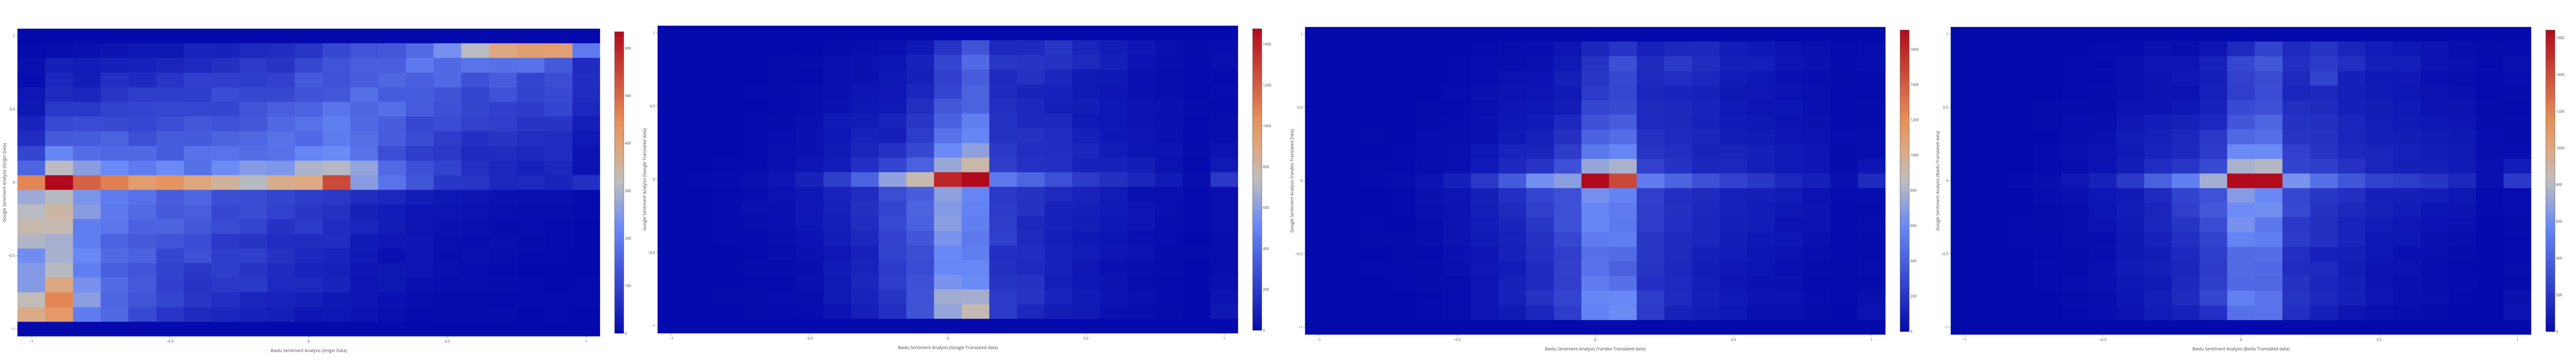
\includegraphics[width=.9\linewidth]{../img/heatmap.png}
\end{center}

% An example of a floating figure using the graphicx package.
% Note that \label must occur AFTER (or within) \caption.
% For figures, \caption should occur after the \includegraphics.
% Note that IEEEtran v1.7 and later has special internal code that
% is designed to preserve the operation of \label within \caption
% even when the captionsoff option is in effect. However, because
% of issues like this, it may be the safest practice to put all your
% \label just after \caption rather than within \caption{}.
%
% Reminder: the "draftcls" or "draftclsnofoot", not "draft", class
% option should be used if it is desired that the figures are to be
% displayed while in draft mode.
%
%\begin{figure}[!t]
%\centering
%\includegraphics[width=2.5in]{myfigure}
% where an .eps filename suffix will be assumed under latex, 
% and a .pdf suffix will be assumed for pdflatex; or what has been declared
% via \DeclareGraphicsExtensions.
%\caption{Simulation results for the network.}
%\label{fig_sim}
%\end{figure}

% Note that the IEEE typically puts floats only at the top, even when this
% results in a large percentage of a column being occupied by floats.


% An example of a double column floating figure using two subfigures.
% (The subfig.sty package must be loaded for this to work.)
% The subfigure \label commands are set within each subfloat command,
% and the \label for the overall figure must come after \caption.
% \hfil is used as a separator to get equal spacing.
% Watch out that the combined width of all the subfigures on a 
% line do not exceed the text width or a line break will occur.
%
%\begin{figure*}[!t]
%\centering
%\subfloat[Case I]{\includegraphics[width=2.5in]{box}%
%\label{fig_first_case}}
%\hfil
%\subfloat[Case II]{\includegraphics[width=2.5in]{box}%
%\label{fig_second_case}}
%\caption{Simulation results for the network.}
%\label{fig_sim}
%\end{figure*}
%
% Note that often IEEE papers with subfigures do not employ subfigure
% captions (using the optional argument to \subfloat[]), but instead will
% reference/describe all of them (a), (b), etc., within the main caption.
% Be aware that for subfig.sty to generate the (a), (b), etc., subfigure
% labels, the optional argument to \subfloat must be present. If a
% subcaption is not desired, just leave its contents blank,
% e.g., \subfloat[].


% An example of a floating table. Note that, for IEEE style tables, the
% \caption command should come BEFORE the table and, given that table
% captions serve much like titles, are usually capitalized except for words
% such as a, an, and, as, at, but, by, for, in, nor, of, on, or, the, to
% and up, which are usually not capitalized unless they are the first or
% last word of the caption. Table text will default to \footnotesize as
% the IEEE normally uses this smaller font for tables.
% The \label must come after \caption as always.
%
%\begin{table}[!t]
%% increase table row spacing, adjust to taste
%\renewcommand{\arraystretch}{1.3}
% if using array.sty, it might be a good idea to tweak the value of
% \extrarowheight as needed to properly center the text within the cells
%\caption{An Example of a Table}
%\label{table_example}
%\centering
%% Some packages, such as MDW tools, offer better commands for making tables
%% than the plain LaTeX2e tabular which is used here.
%\begin{tabular}{|c||c|}
%\hline
%One & Two\\
%\hline
%Three & Four\\
%\hline
%\end{tabular}
%\end{table}


% Note that the IEEE does not put floats in the very first column
% - or typically anywhere on the first page for that matter. Also,
% in-text middle ("here") positioning is typically not used, but it
% is allowed and encouraged for Computer Society conferences (but
% not Computer Society journals). Most IEEE journals/conferences use
% top floats exclusively. 
% Note that, LaTeX2e, unlike IEEE journals/conferences, places
% footnotes above bottom floats. This can be corrected via the
% \fnbelowfloat command of the stfloats package.




\section{Conclusion}
The conclusion goes here.




% conference papers do not normally have an appendix



% use section* for acknowledgment
\ifCLASSOPTIONcompsoc
  % The Computer Society usually uses the plural form
  \section*{Acknowledgments}
\else
  % regular IEEE prefers the singular form
  \section*{Acknowledgment}
\fi


The authors would like to thank...





% trigger a \newpage just before the given reference
% number - used to balance the columns on the last page
% adjust value as needed - may need to be readjusted if
% the document is modified later
%\IEEEtriggeratref{8}
% The "triggered" command can be changed if desired:
%\IEEEtriggercmd{\enlargethispage{-5in}}

% references section

% can use a bibliography generated by BibTeX as a .bbl file
% BibTeX documentation can be easily obtained at:
% http://mirror.ctan.org/biblio/bibtex/contrib/doc/
% The IEEEtran BibTeX style support page is at:
% http://www.michaelshell.org/tex/ieeetran/bibtex/
%\bibliographystyle{IEEEtran}
% argument is your BibTeX string definitions and bibliography database(s)
%\bibliography{IEEEabrv,../bib/paper}
%
% <OR> manually copy in the resultant .bbl file
% set second argument of \begin to the number of references
% (used to reserve space for the reference number labels box)
\begin{thebibliography}{1}

\bibitem{IEEEhowto:kopka}
H.~Kopka and P.~W. Daly, \emph{A Guide to \LaTeX}, 3rd~ed.\hskip 1em plus
  0.5em minus 0.4em\relax Harlow, England: Addison-Wesley, 1999.

\end{thebibliography}




% that's all folks
\end{document}


